\documentclass[12pt]{article}
\usepackage[english]{babel}
\usepackage[a4paper,top=2cm,bottom=2cm,left=3cm,right=3cm,marginparwidth=1.75cm]{geometry}

\usepackage{float}
\usepackage{amsmath}
\usepackage{graphicx}
\usepackage[colorlinks=true, allcolors=blue]{hyperref}

\title{Installing Python and Jupyter Notebook}
\date{}
\begin{document}
\maketitle

% \vspace{-1cm}
\noindent All course material will be written in Python 3.

\section{I already have Python}
If you already have Python installed and if you are familiar with installing
Python packages with \verb|pip|, you can use this to install Jupyter. Please make
sure you that you have upgraded to the latest version of \verb|pip| using the following command: \\

\verb|pip3 install --upgrade pip| \\

\noindent Next install the Jupyter notebook with: \\

\verb|pip3 install jupyter| \\

\noindent In this course we will use many external packages that need to be installed. To manage them smoothly, you are recommended to use the \textbf{Anaconda} Python distribution. If you
do not have Anaconda installed, please see Section 2 for how to install it.
If you already have Anaconda installed, please go to Section 3 to create a
virtual environment with all the required packages for this module.

\section{I am new to Python}
    \subsection{Download Anaconda}
    Anaconda is a Python distribution for data science and machine learning.
    It can be freely downloaded \href{https://www.anaconda.com/products/individual-d}{here}.
    
    \subsection{Install Anaconda}
    Follow \href{https://docs.anaconda.com/anaconda/install/}{these instructions} to install Anaconda distribution on your computer. The instructions support Windows, Mac and Linux.
    
    % \newpage
    \subsection{Test the installation}
    Jupyter notebook should now be successfully installed on your local machine. Please open a new terminal window with one of the commands below: \\

    \noindent \textbf{Windows}: press \verb|[WIN]+[r]| and type \verb|cmd|. Then press \verb|[Enter]|. \\
    \textbf{Mac}: press \verb|[command]+[space]| to open Spotlight. Then type terminal
    and press \verb|[enter]|. \\
    \textbf{Linux}: in Unity/Gnome press \verb|[Ctrl]+[Alt]+[T]|. \\
    
    \noindent Type the following command in terminal to run the notebook. \\
    
    \verb|jupyter notebook| \\
    
    \noindent This should open a browser and a webpage that looks similar to the illustration in Figure 1. (It is possible that the webpage shown on your local machine make look slightly different).
    
    \begin{figure}[H]
        \centering
        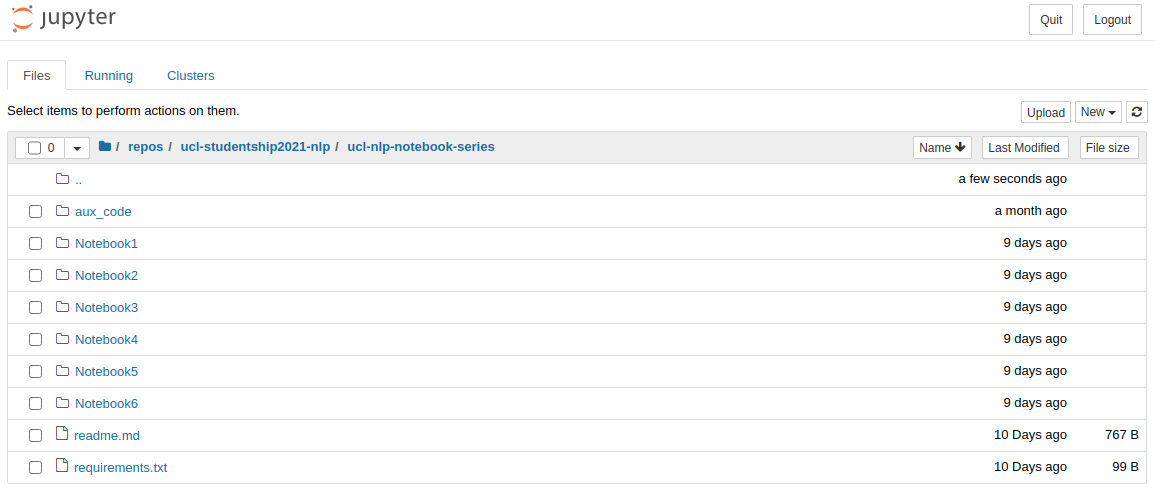
\includegraphics[width=\textwidth]{"img/pic.png"}
        \caption{Jupyter notebook in browser}
    \end{figure}
    
\section{Create virtual environment}
A virtual environment is a named, isolated, working copy of Python that that maintains its own files, directories, and paths so that you can work with specific versions of libraries or Python itself without affecting other Python projects.

To create a new virtual environment that contains all packages needed for this module and a stable Python version please run the following two commands (replace \verb|*name*| with your preferred name): \\

\verb|conda create --name *name* python=3.8.10 numpy pandas scipy|\\
\indent \verb|scikit-learn matplotlib seaborn gensim=4.0.1 spacy nltk| \\

\verb|conda install --name *name* -c conda-forge notebook ipykernel| \\
\indent \verb|langdetect swifter imbalanced-learn emoji| \\

\noindent To activate your newly created virtual environment, run the following command: \\

\verb|conda activate *name*| \\

\noindent We need to install one more thing, this time using \verb|pip|. After activating your virtual environment run: \\

\verb|pip3 install PyMuPDF| \\


\vspace{-0.5cm}
\section{Check package versions}
You can check the versions of the installed packages by opening up a notebook, importing all the packages and checking the \verb|__version__| attribute. \\

\verb|import numpy as np| \\

\verb|np.__version__| \\

Below you can see the versions for each package that guarantee the notebooks to run smoothly:
\begin{itemize}
    \item matplotlib == 3.4.2
    \item numpy == 1.20.3
    \item pandas == 1.3.0
    \item gensim == 4.0.1
    \item PyMuPDF == 1.18.17
    \item spacy == 2.3.5
    \item scikit-learn == 0.24.2
    \item nltk == 3.6.2
    \item seaborn == 0.11.2
    \item swifter == 1.0.9
    \item langdetect == 1.0.9
    \item imbalanced-learn == 0.8.0
    \item emoji == 1.4.2
    \item ipykernel == 6.3.1
    \item notebook == 6.4.3
\end{itemize}

\end{document}